\begin{frame}[fragile] 
%--------------------------------------------------
\frametitle{\cello\ Software Design}
\framesubtitle{Component diagram}
%--------------------------------------------------
\centerline{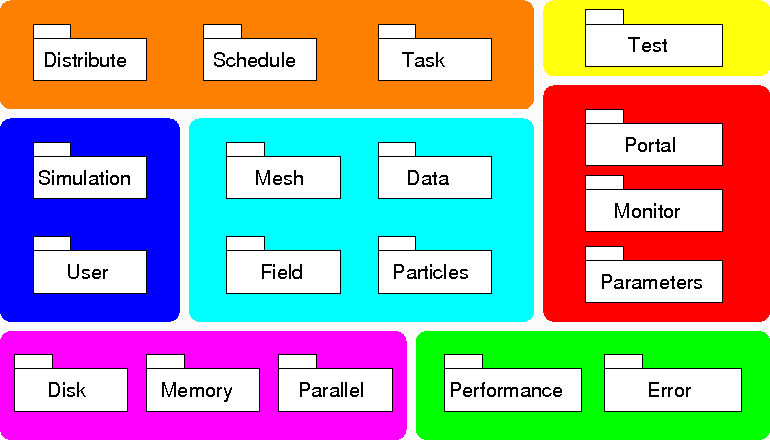
\includegraphics[width=4in]{components4.png}}
\end{frame}

\begin{frame}[fragile] 
%--------------------------------------------------
\frametitle{\cello\ Software Design}
\framesubtitle{Component diagram}
%--------------------------------------------------

\begin{tabbing}
xxx\=xxxxxxxxxxxxxxxx\=\kill
\> \enhance{1} {\color{orange} Parallel} \> distribute and schedule parallel tasks \\
\> \enhance{1} {\color{blue} Methods} \> solvers and simulation specification \\
\> \enhance{1} {\color{cyan} Data} \> methods and data structures \\
\> \enhance{1} {\color{magenta} Hardware} \> interact with middleware and hardware \\
\> \enhance{1} {\color{red} Interface} \> interface with users and other software \\
\> \enhance{1} {\color{green} Cross-cutting} \> performance monitoring and error-handling
\end{tabbing}

\begin{itemize}
\enhance{2}\item One source code directory per component, e.g. \code{src/Field/}
\enhance{3}\item Access a component using, e.g., \code{\#include "parallel.hpp"}
\end{itemize}
\end{frame}


\begin{frame}[fragile] 
%--------------------------------------------------
\frametitle{\cello\ Software Design}
\framesubtitle{\code{Field} component}
%--------------------------------------------------

The \colorcode{Field} component represents data fields at the block level

\begin{itemize}
 \enhance{2}\item Data layout parameterized (ordering, padding, alignment)
 \enhance{3}\item Field groups can be defined
\begin{itemize}
 \enhance{3}\item     generalization of color fields
\end{itemize}
 \enhance{4}\item Floating point precision
\begin{itemize}
 \enhance{4}\item    \code{Field \{ precision = "extended96" \}}
\end{itemize}
 \enhance{5}\item Ghost zones
\begin{itemize}
 \enhance{5}\item    \code{Field \{ ghosts = [3,3,3] \}}
\end{itemize}
 \enhance{6}\item Minimum/maximum handling
\begin{itemize}
 \enhance{6}\item    \code{Field \{ pressure \{ minimum = [1e-6,"warning"] \} \} }
\end{itemize}
\end{itemize}
\end{frame}

\begin{frame}[fragile] 
%--------------------------------------------------
\frametitle{\cello\ Software Design}
\framesubtitle{\code{User} component}
%--------------------------------------------------

The \colorcode{User} component is where \enzo\ kernels live \ \\
\ \\
\footnotesize
\begin{tabular}{ll}
      \code{UserMethod} &    methods, initialization, analysis functions \\
      \code{UserCorrect} &  flux-correction type operations \\
      \code{UserBoundary} &  specialized boundary conditions \\
      \code{UserTimestep} &  specialized timestep control \\
      \code{UserRefinement} & specialized refinement criteria \\
      \code{UserBalance}  &  specialized load balancing \\
      \code{UserSchedule} &  specialized task scheduling
\end{tabular}
\end{frame}

\begin{frame}[fragile] 
%--------------------------------------------------
\frametitle{\cello\ Software Design}
\framesubtitle{\code{Portal} component}
%--------------------------------------------------
The \colorcode{Portal} component serves to interact with external codes \\
\begin{itemize}
\item\enhance{1} Inter-application communication analogous to \code{Parameters}
\begin{itemize}
\item\enhance{1}    probably XML-based
\item\enhance{1}    two-way communication
\end{itemize}
\item\enhance{2} Example uses
\begin{itemize}
\item\enhance{3} modify method or AMR parameters
\item\enhance{4} control a virtual ``camera''
\item\enhance{6} dynamic data analysis
\item\enhance{7} plug in jacques, yt, etc.
\end{itemize}
\end{itemize}
\end{frame}
% PORTAL COMPONENT
%
%  * interact with external utilities
%    - yt, jacques, etc.
%  - inter-application communication using Parameters-like API
%    - probably XML
%    - read commands to retrieve data
%    - write commands to control simulation
%  * Example uses
%    - control
%      - modify simulation parameters as it progresses
%      - maintain log so results can be reproduced
%    - locate
%      - dynamically look for and track features
%    - analyse
%    - visualize
%      - e.g. contral a dynamic camera position, direction, frequency sensitivity, etc.
%    - performance
%      - find performance problems
%      - dynamically modify parameters to correct
%
%  * user-driven dynamic analysis
%    - more efficient than a posteriori analysis
%      - no large disk dumps
%    - more flexible than inline analysis
%      - discover and analyse features at run time
%      - all data available
%    - can dynamically change what data to store for later analysis
%      - useful if analysis would otherwise slow the computation
%
